\documentclass[border=10pt]{standalone}
\usepackage{tikz}\usepackage{amsmath}\usetikzlibrary{arrows.meta}
\begin{document}
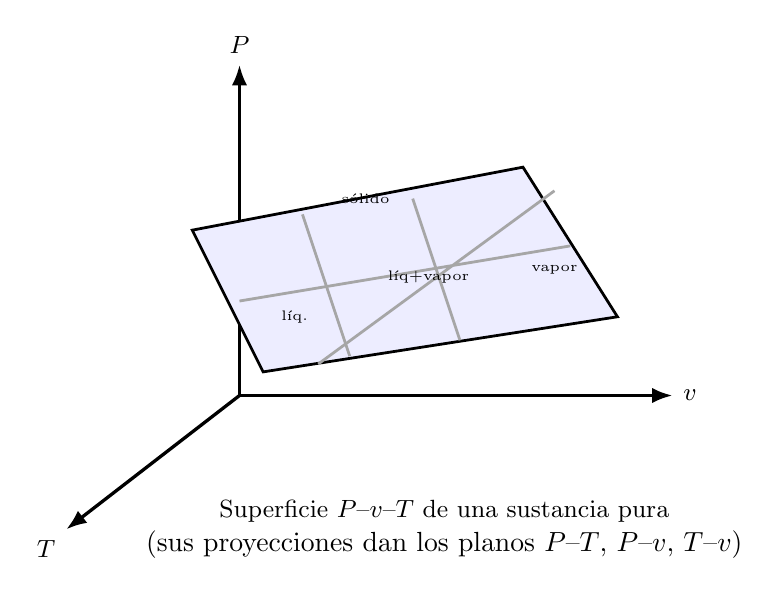
\begin{tikzpicture}[line width=1pt,>={Latex[length=2.6mm]}]
  % ejes pseudo-3D
  \draw[->,line width=1.2pt] (0,0)--(0,4.2) node[above]{\small $P$};
  \draw[->,line width=1.2pt] (0,0)--(5.5,0) node[right]{\small $v$};
  \draw[->,line width=1.2pt] (0,0)--(-2.2,-1.7) node[below left]{\small $T$};
  % superficie esquematica (parche)
  \fill[blue!7] (0.3,0.3)--(4.8,1.0)--(3.6,2.9)--(-0.6,2.1)--cycle;
  \draw[line width=1.0pt] (0.3,0.3)--(4.8,1.0)--(3.6,2.9)--(-0.6,2.1)--cycle;
  % lineas de malla
  \draw[black!35] (1.4,0.5)--(0.8,2.3) (2.8,0.7)--(2.2,2.5);
  \draw[black!35] (0.0,1.2)--(4.2,1.9) (1.0,0.4)--(4.0,2.6);
  % regiones
  \node at (0.7,1.0){\tiny líq.};
  \node at (2.4,1.5){\tiny líq+vapor};
  \node at (4.0,1.6){\tiny vapor};
  \node at (1.6,2.5){\tiny sólido};
  \node[align=center] at (2.6,-1.7){\small Superficie $P$--$v$--$T$ de una sustancia pura\\(sus proyecciones dan los planos $P$--$T$, $P$--$v$, $T$--$v$)};
\end{tikzpicture}
\end{document}
